\documentclass{beamer}
\usepackage[utf8]{inputenc}
\usetheme{Madrid}

\title{Optimización Bayesiana en Antenas}
\subtitle{Data-Driven Bayesian Optimization Framework for Rapidly Developing Novel Wideband, Low-Profile Dipole Antenna With 3-D-Printed Technology}
\author{Nicolás Seguel}
\date{\today}

\begin{document}

\frame{\titlepage}

% --- Problema ---
\begin{frame}{Problema estudiado}
  \begin{itemize}
    \item Se busca diseñar una antena dipolo compacta, de bajo perfil y un gran ancho de banda (BW).
    \item Problema: el diseño de la antena es demasiado complejo para afinarla a partir de prueba y error.
    \item Simulaciones electromagnéticas (CST) son costosas, con tiempos de evaluación de 10-15 minutos.
    \item Espacio de diseño de alta dimensión (20 variables).
    \item Métodos tradicionales (PSO, TRF) no logran convergencia eficiente.
  \end{itemize}
\end{frame}

% --- Antena ---
\begin{frame}{Estructura de la antena}
  \begin{columns}
    \column{0.5\textwidth}
      \centering
      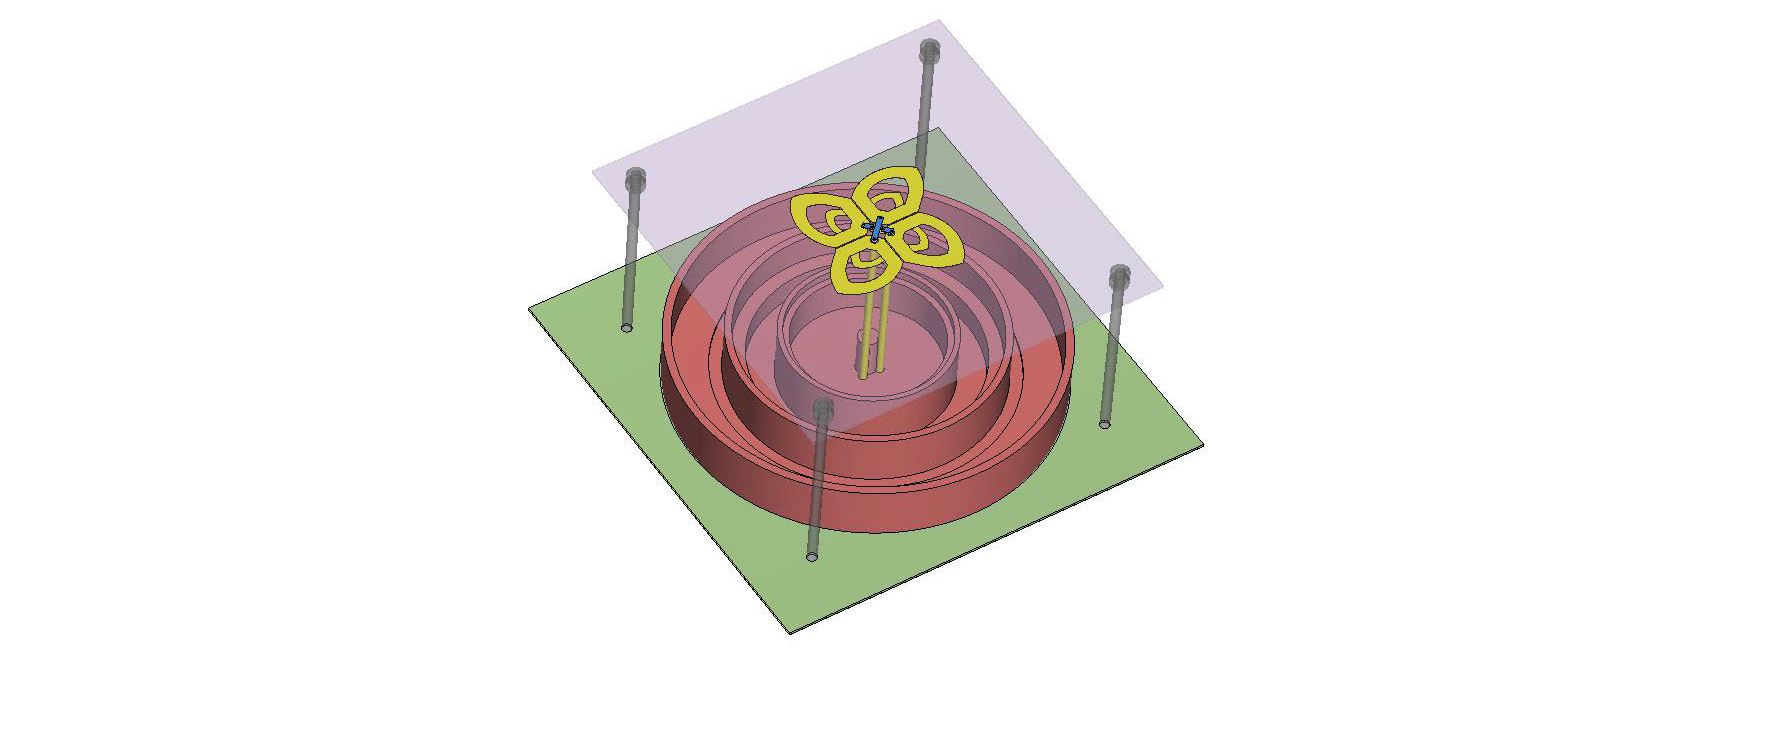
\includegraphics[width=1.2\textwidth]{antenna.png} % <-- pon aquí tu imagen exportada del paper o CST
    \column{0.5\textwidth}
      \begin{itemize}
        \item Dipolo cruzado en forma de pétalo.
        \item 10 capas de material dieléctrico de alta permitividad (HDL).
        \item Variables de diseño: alturas $h_i$ y radios $r_i$.
      \end{itemize}
  \end{columns}
\end{frame}

% --- Introducción a BO ---
\begin{frame}{Optimización Bayesiana (BO)}
  \begin{itemize}
    \item Técnica para optimizar funciones desconocidas:
      \begin{itemize}
        \item Costosas de evaluar.
        \item Sin gradiente analítico.
        \item Posiblemente no convexas.
      \end{itemize}
    \item Idea principal:
      \begin{enumerate}
        \item Construir un \textbf{modelo probabilístico} (sustituto) de la función objetivo.
        \item Usar una \textbf{función de adquisición} para decidir dónde muestrear siguiente.
        \item Actualizar el modelo con cada nueva evaluación.
      \end{enumerate}
    \item Ventaja: requiere muchas menos evaluaciones que una búsqueda exhaustiva o heurística.
  \end{itemize}
\end{frame}

% --- Función objetivo ---
\begin{frame}{Modelo de optimización}
  Variables de diseño:
  \[
    x = \{h_1,\dots,h_{10}, r_1,\dots,r_{10}\}
  \]
  Función objetivo (\textbf{Ecuación (6)}):
  \[
  f(x) = f_1(x) + f_2(x) + f_3(x)
  \]
  \begin{itemize}
    \item $f_1(x) = \sum_{w=w_1}^{w_2} \max(0, g_{S11}(\textbf{x},w)-T_{S11})$ (donde $T_{S11}=-15$ dB)
    \item $f_2(x) = \sum_{w=w_1}^{w_2} \max(0, g_{S21}(\textbf{x},w)-T_{S21})$ (donde $T_{S21}=-20$ dB)
    \item $f_3(x) = \sum_{w=w_1}^{w_2} \max(0, T_{gain} - g_{gain}(\textbf{x},w))$ (donde $T_{gain}=6$ dB)
  \end{itemize}
\end{frame}

% --- Tree-structured Parzen Estimator (TPE) ---
\begin{frame}{Tree-structured Parzen Estimator (TPE)}
  \begin{itemize}
    \item Variante de BO que modela \textbf{$p(x|y)$} en lugar de $p(y|x)$.
    \item Divide los resultados en dos grupos:
      \begin{itemize}
        \item $D^{(l)}$: diseños ``buenos'' (valores por debajo de un umbral $\gamma$).
        \item $D^{(g)}$: diseños ``malos'' (el resto).
      \end{itemize}
    \item Ajusta dos distribuciones de densidad (KDEs):
      \[
        l(x) = p(x|D^{(l)}), \quad g(x) = p(x|D^{(g)})
      \]
    \item Escoge nuevos puntos maximizando la razón:
      \[
        r(x) = \frac{l(x)}{g(x)}
      \]
  \end{itemize}
\end{frame}


% --- Algoritmo ---
\begin{frame}{Método TPE-BO}
    \begin{columns}
      \column{0.5\textwidth}
        \centering
        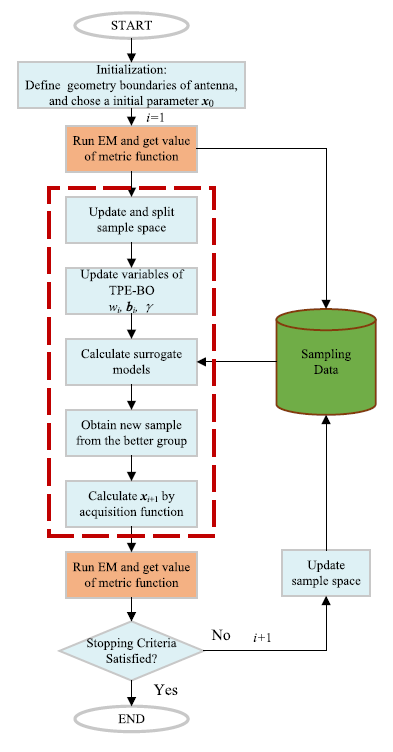
\includegraphics[height= 0.8\textheight]{tpe_flow.png} % <-- diagrama de flujo del algoritmo
      \column{0.5\textwidth}
        \centering
        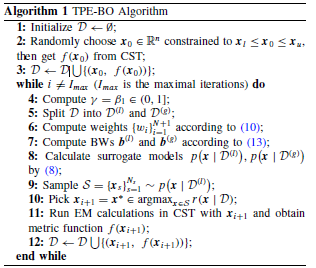
\includegraphics[width= 0.8\textwidth]{algoritm.png}
    \end{columns}
\end{frame}

% --- Resultados en punteo ---
\begin{frame}{Resultados principales}
  \begin{itemize}
    \item Ancho de banda solapado: 1.62-3.75 GHz (79.3\%).
    \item Perfil reducido: $0.2\lambda \rightarrow 0.1\lambda$.
    \item $VSWR < 1.6$ en la banda de operación.
    \item Aislamiento $> 20.5$ dB.
    \item Óptimo en 700 iteraciones (10-15 min c/u).
  \end{itemize}
\end{frame}

% --- Resultados gráficos ---
\begin{frame}{Resultados experimentales}
  \begin{columns}
    \column{0.5\textwidth}
        \centering
        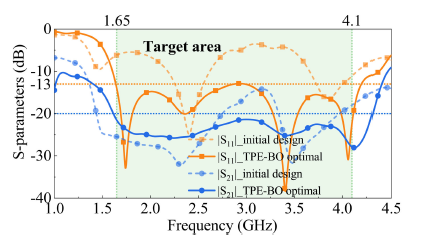
\includegraphics[width=0.8\linewidth]{s_plot.png} \\[-0.2cm]
        \centering \scriptsize Resultados obtenidos con el algoritmo TPE-BO
    \column{0.5\textwidth}
        \centering
        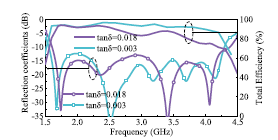
\includegraphics[width=0.8\linewidth]{hdl_eff.png} \\[-0.2cm]
        \centering \scriptsize Comparación de eficiencia entre diferentes materiales HDL
  \end{columns}
  \begin{columns}
    \column{0.5\textwidth}
        \centering
        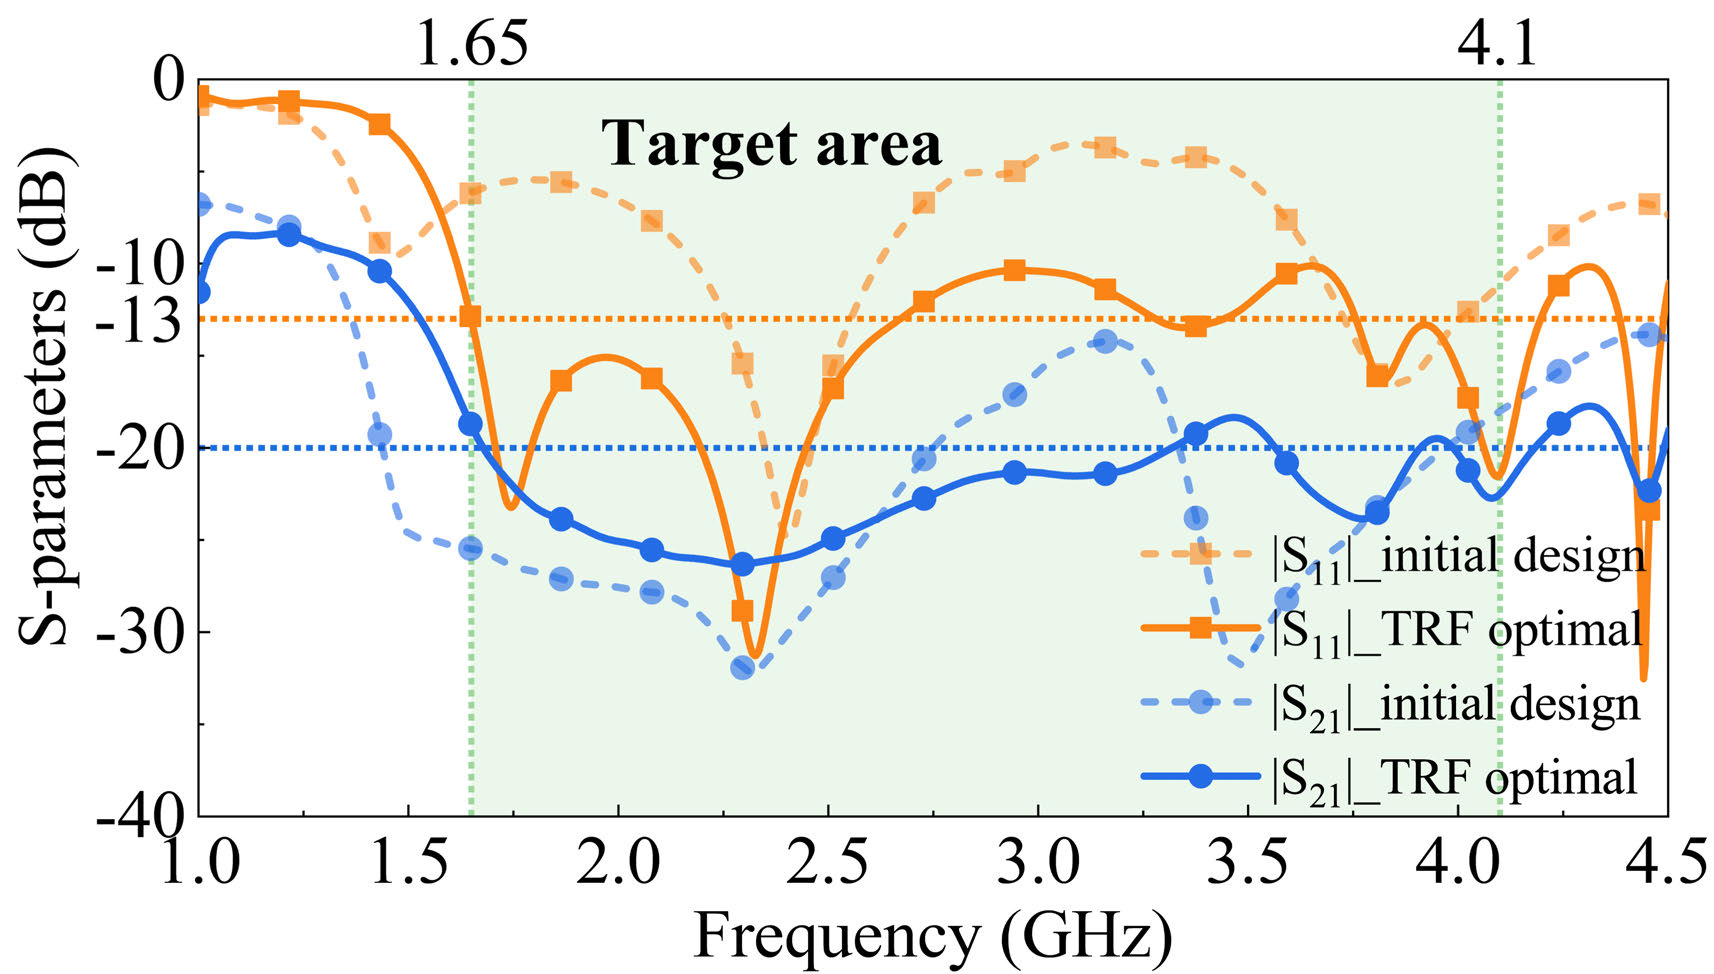
\includegraphics[width=0.8\linewidth]{TRF.png} \\
        \scriptsize Resultados con el método TRF
    \column{0.5\textwidth}
        \centering
        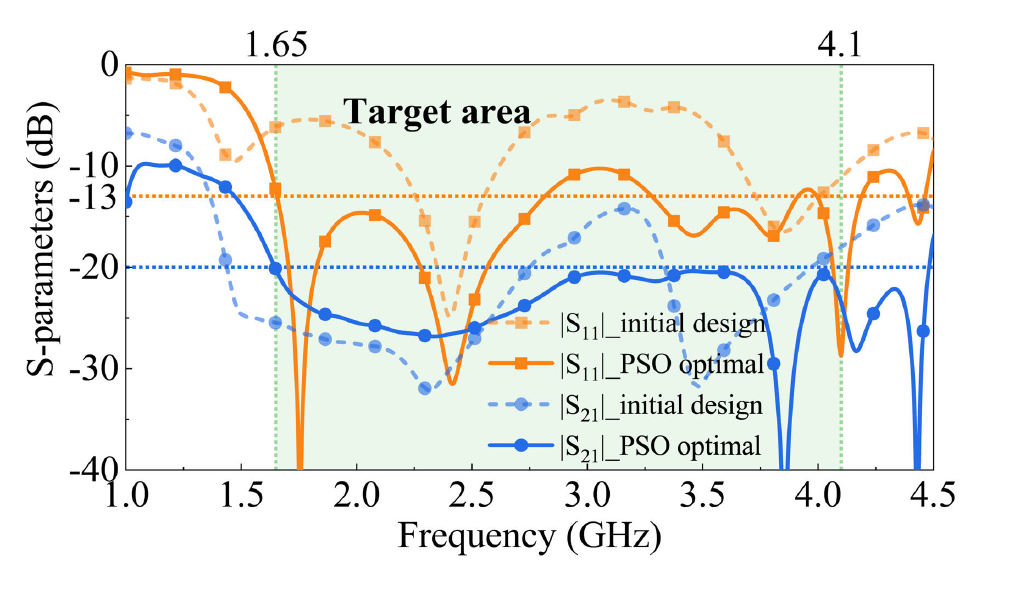
\includegraphics[width=0.8\linewidth]{PSO.png} \\
        \scriptsize Resultados con el método PSO
  \end{columns}
\end{frame}


% --- Conclusiones ---
\begin{frame}{Conclusiones}
  \begin{itemize}
    \item El marco TPE-BO permitió diseñar de forma rápida y eficiente una antena dipolo de bajo perfil y gran ancho de banda.
    \item El prototipo alcanzó un ancho de banda solapado de 79.3\% y un perfil reducido a 0.1$\lambda$.
    \item La impresión 3D con materiales HDL validó la factibilidad del diseño en la práctica.
    \item La estrategia presentada es una solución viable para el diseño de antenas complejas en espacios de alta dimensión.
  \end{itemize}
\end{frame}


\end{document}